\documentclass[journal]{IEEEtran}
\usepackage[cmex10]{amsmath}
\usepackage{algorithm}% http://ctan.org/pkg/algorithms
\usepackage{graphicx}
\usepackage{algpseudocode}% http://ctan.org/pkg/algorithmicx
\usepackage{array}
\usepackage{url}
\usepackage{flushend}
\usepackage[caption=false,font=footnotesize]{subfig}

\providecommand{\todo}[1]{{\protect\color{black}{[\textbf{Comment:} #1]}}}
\providecommand{\TODO}[1]{{\protect\color{black}{[\textbf{Comment:} #1]}}}
\providecommand{\rv}[1]{{\protect\color{black}{#1}}}
\providecommand{\rrv}[1]{{\protect\color{black}{#1}}}
\providecommand{\bmark}[1]{{\protect\color{black}{#1}}}
\usepackage{amsfonts}

\newcommand{\tickYes}{\checkmark}
\usepackage{pifont}
\newcommand{\tickNo}{\hspace{1pt}\ding{55}}

\usepackage[latin1]{inputenc}
\usepackage{multirow}
\usepackage{amssymb}
\hyphenation{op-tical net-works semi-conduc-tor}

\usepackage{siunitx}
\usepackage{color}
\usepackage{cite}
\usepackage{colortbl}
\usepackage[table]{xcolor}
\usepackage{booktabs}
\usepackage{datetime}

\newcommand{\REVIEW}[1]{\textcolor{red}{\bf{\raggedright{\textsf{REVIEW: #1\\}}}}}

\setlength{\heavyrulewidth}{0.1em}
\newcommand {\otoprule}{\midrule[\heavyrulewidth]}
\renewcommand{\arraystretch}{1.1}

\sloppy
\tolerance=999
\renewcommand\floatpagefraction{.9}
\renewcommand\topfraction{.9}
\renewcommand\bottomfraction{.9}
\renewcommand\textfraction{.1}   
\setcounter{totalnumber}{50}
\setcounter{topnumber}{50}
\setcounter{bottomnumber}{50}

\begin{document}
\title{\rv{Using Visual Rhythms for Detecting\\Video-based Facial Spoof Attacks}}
\author{Allan~Pinto,
        William~Robson~Schwartz,
        Helio~Pedrini, and 
        Anderson~Rocha
\thanks{Manuscript received March X, XXX; revised March XX, XXXX.}}

% The paper headers
\markboth{IEEE TRANSACTIONS ON INFORMATION FORENSICS AND SECURITY,~Vol.~XX, No.~XX, March~XXXX}%
{Shell \MakeLowercase{\textit{et al.}}: Bare Demo of IEEEtran.cls for Journals}

\maketitle

\begin{abstract}
\rv{Spoofing attacks or impersonation} can be easily accomplished in a facial biometric system wherein users without access privileges attempt to authenticate themselves as valid users, in which an impostor needs only a photograph or a video with facial information of a legitimate user. Even with recent advances in biometrics, information forensics and security, vulnerability of facial biometric systems against \rv{spoofing attacks} is still an open problem. Even though several methods have been proposed for photo-based spoofing attack detection, attacks performed with videos have been vastly overlooked, which hinders the use of the facial biometric systems in modern applications. In this paper, we present an algorithm for video-based spoofing attack detection through the analysis of global information which is invariant to content, since we discard video contents and analyze content-independent noise signatures present in the video related to the unique acquisition processes. Our approach takes advantage of noise signatures generated by the recaptured video to distinguish between fake and valid access videos. For that, we use the Fourier spectrum followed by the computation of video visual rhythms and the extraction of different characterization methods. For evaluation, we consider the novel Unicamp Video-Attack Database (UVAD) which comprises 17,076 videos composed of real access and spoofing attack videos. In addition, we evaluate the proposed method using the Replay-Attack Database, which contains photo-based and video-based face spoofing attacks.
\end{abstract}

\begin{IEEEkeywords}
Video-based Face Spoofing, Visual Rhythm, Video-based Attacks, Unicamp Video-Attack Database; \rv{Impersonation Detection in Facial Biometric Systems.}
\end{IEEEkeywords}

\IEEEpeerreviewmaketitle

\section{Introduction}
\label{Introduction}

\IEEEPARstart{B}{iometric} authentication is an important mechanism for access control that has been used in many applications. Traditional \rv{methods, including the ones based on knowledge (e.g., keywords, secret question) or based on tokens (e.g., smart cards), might be ineffective since they are easily shared,} lost, stolen or manipulated. In contrast, the biometric access control has been shown as a natural and reliable authentication method~\cite{Jain:HB:2008}.

Access control can be seen as a verification problem wherein the authentication of a user is performed by reading and comparing the input biometric data captured by an acquisition sensor (query) with the biometric data of the same user previously stored in a database (template). The comparison between the query and the template is performed by a matching algorithm which produces a similarity score used to decide whether or not the access should be granted to the user.

Although biometric authentication is considered a secure and reliable access control mechanism, it becomes an easy target for attacks if protective measures are not implemented. \rrv{Fig.}~\ref{biometricsystem} shows a general biometric authentication system without any protective measure and some points of vulnerabilities. Buhan et al.~\cite{Buhan:CTITUT:2005} provide more details about abuses in biometric systems. 

\begin{figure}[!htb]
\centering
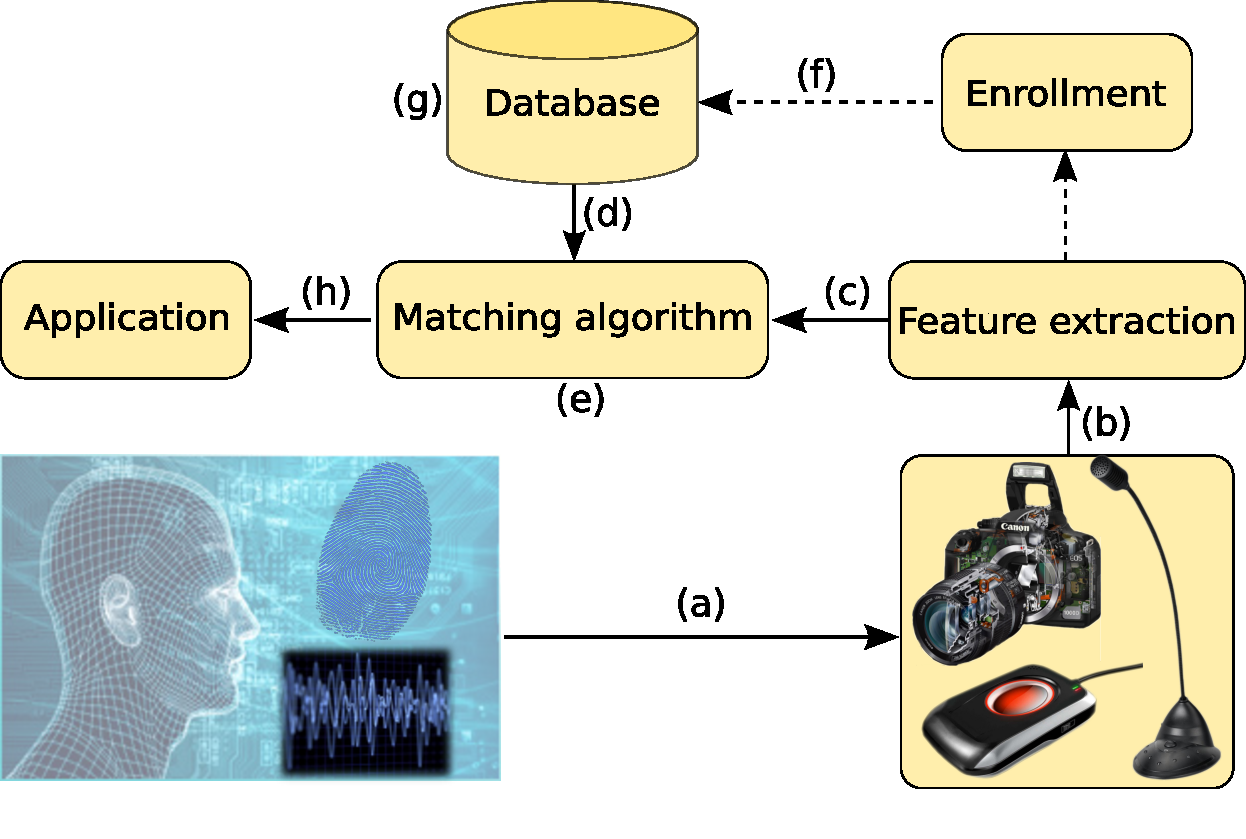
\includegraphics[width=0.3\textwidth]{figure-01.pdf}
\caption{General biometric system and its vulnerability points. (a) a threat resulting from an attack on the biometric sensor, presenting a synthetic biometric data (fake); (b), (c) and (d) represent threats resulting from re-submission of a biometric latent signal previously stored in the communication channel; (e) attack on the matching algorithm in order to produce a higher or lower score; (f) an attack on the communication channel between the enrollment center and the database (\rv{the  control} of this channel allows an attacker to overwrite the template that is sent to the biometric database); (g) an attack on the database itself, which could result in corrupted models, denial of service to the person associated to the corrupted model, or fraudulent authorization of an individual; (h) an attack that consists of overwriting the output of the matching algorithm, bypassing the authentication process.}
\label{biometricsystem}
\end{figure}

Spoofing attack is a type of attack wherein an impostor presents a fake biometric data to the acquisition sensor with the goal of authenticating oneself as a legitimate user (\rv{this action can be seen as an impersonation attack}), illustrated in \rrv{Fig.}~\ref{biometricsystem}(a). Depending on the biometric trait used by the system, this mode of attack can be easily accomplished because some biometric data can be synthetically reproduced without much effort. Face biometric systems are highly vulnerable to such attacks since facial traits are widely available on the Internet, on personal websites and social networks such as Facebook\footnote{\url{http://www.facebook.com}}, MySpace\footnote{\url{http://www.myspace.com}}, YouTube\footnote{\url{http://www.youtube.com}}. In addition, we can easily collect facial samples of a person \rv{with} a digital camera.

In the context of face biometrics, \bmark{a spoofing attack can be attempted by} presenting to the acquisition sensor a photograph, a video or a 3D face model of a legitimate user enrolled in the database. If an impostor succeeds in the attack using any of these approaches, the \rv{uniqueness premise of the biometric system or its \emph{raison d'\^etre} is violated}, making the system vulnerable~\cite{Jain:HB:2008}.

Several methods have been proposed in the literature to detect spoofing attacks based on photographs, whereas attacks performed with videos and 3D models have been overlooked. Many methods aim at distinguishing real from fake biometric data based on the fact that artifacts are inserted into the printed samples due to printing process, therefore allowing one to explore attributes related to such artifacts including color, shape and texture~\cite{Tan:ECCV:2010,Maatta:IJCB:2011,Schwartz:IJCB:2011}. Since photographs are static, another approach is to detect small movements in the face~\cite{Pan:ICCV:2007,Li:ICMLC:2008,Xu:ICIP:2008}. Recent works~\cite{Pan:TS:2011,Anjos:IJCB:2011} investigate context information of the scene (e.g., background information) to detect face liveness.

We believe that the aforementioned approaches are not suitable for detecting video-based attacks directly, especially in high resolution videos. The difficulty in detecting spoofing performed by video lies in the fact that it is easier to deceive an authentication system through a video since the dynamics of the video makes the biometric data more realistic. Furthermore, the content of a video is less affected by degradations in terms of color, shape or texture, unlike the printed images. Finally, we have less artifacts generated during quantization and discretization of the image captured by the imaging sensor in high resolution videos.

In this paper, we present a method for detecting video-based face spoofing attacks under the hypothesis that fake and real biometric data contain different acquisition-related noise signatures. To the best of our knowledge, this is the first attempt of dealing with video-based face spoofing using analysis of global information that is invariant to the video content. Our solution explores the artifacts added to the biometric samples during the viewing process of the videos in the display devices and noise signatures added during the recapture process performed by the acquisition sensor of the biometric system. Through the spectral analysis of the noise signature and the use of visual rhythms, we designed a feature characterization process able to incorporate temporal information of the behavior of the noise signal from the biometric samples.

In a previous work~\cite{Pinto:SIBGRAPI:2012}, we introduced an anti-spoofing solution that was evaluated in an extended version of the Print-Attack database~\cite{Anjos:IJCB:2011} \rv{given that, in the literature,} there was no specific database to video-based face spoofing attacks. Originally, the Print-Attack database was developed to be used in the evaluation of photograph-based spoofing attack detection. 
%being composed of $200$ videos of valid access of $50$ identities and $200$ videos of attempted spoofing attack using printed photographs captured with a generic webcam with $ 320 \times 240$ pixel resolution. 
As our aim in that work was also at video-based spoofing detection, we simulated attempts of spoofing \rv{attacks} using $100$ videos of valid access in six monitors, generating $600$ attempted attack videos. We reported near-perfect classification results ($\textrm{AUC} \approx 100\%$). That is due to the low resolution of original videos, which favored the high performance of our method, since noise signal \rv{was} the main information used in it. Furthermore, in a more realistic attack, an impostor probably would create fake biometric samples with the highest quality possible in order to minimize the differences between real and fake biometric samples. 

To contemplate a more realistic scenario, this work extends upon our previous work~\cite{Pinto:SIBGRAPI:2012} and also introduces the Unicamp Video-Based Attack Database (UVAD)\footnote{This database will be make public and freely available. Users present in the database formally authorized the release of their data \rv{for scientific purposes.}}, specifically developed to evaluate video-based attacks in order to verify the following aspects:
%
\begin{itemize}
	\item The behavior of the method for attempted attacks with high resolution videos;
	\item The influence of the display devices in our method;
	\item The influence of the biometric sensor in the proposed method;
	\item The best feature characterization to capture the video artifacts;
	\item Comparison with \bmark{one of the best anti-spoofing} methods for photo-based spoofing attack \rv{of notice}.
\end{itemize}

Such verifications can be accomplished due to the diversity of the devices used to create the database which comprises valid access and attempted attack videos of $404$ different people. Each user was filmed in two sections in different scenarios and lighting conditions. The attempted attack videos were produced using seven different display devices and six digital cameras from different manufacturers. The database has $808$ valid access videos and $16,268$ videos of video-based attempted spoofing attacks, all in full high definition quality. 

\rv{In summary}, the main contributions of this work are:
%
\begin{enumerate}
	\item[(i)] An efficient and effective method for video-based face spoofing attack detection able to recognize attempted attacks carried out with high-resolution videos;
	\item[(ii)] The {evaluation of the video characterization process considering different image features such as} the Gray-Level Co-occurrence Matrices (GLCM), Histograms of Oriented Gradients (HOG) and Local Binary Patterns Histogram (LBP) feature descriptors;
	\item[(iii)] The creation of a \bmark{large and publicly available benchmark} to evaluate anti-spoofing methods performed with videos considering several display devices and different acquisition sensors;
	\item[(iv)] A detailed study of the video-based spoofing attack problem that yielded important conclusions that certainly will be useful for the proposition of new anti-spoofing methods for video-based attacks \rv{not only in the biometric domain but also in other applications analyzing video recapture footprints}.
\end{enumerate}

{We organize the \bmark{remainder of this paper} into five sections. Section~\ref{sec:RelatedWork} discusses state-of-the-art methods for detecting spoofing attacks to face biometrics. Section~\ref{sec:ProposedMethod} presents the proposed method. Section~\ref{sec:DatabaseCreation} gives details regarding the proposed video-attack database while Section~\ref{sec:ExperimentsAndResults} shows and discusses the experimental results. Finally, Section~\ref{sec:Conclusion} presents the conclusions obtained with this work.}

\section{Related Work}
\label{sec:RelatedWork}

According to Pan et al.~\cite{Pan_2008}, there are four major categories of anti-spoofing methods: data-driven characterization, user behavior modeling, user interaction need, and the presence of additional devices. Solutions that require extra devices are limited due to their high cost, which can \bmark{prevent large-scale use} (e.g., deployment of an anti-spoofing solution on all ATMs of a banking network). The user cooperation during the biometric authentication can also be used to facilitate spoofing attack detection, however, this procedure lessens the transparency and inserts an additional time in the authentication process. Finally, the user behavior modeling approach (e.g., eye blinking, small face movements) has been considered in the literature for photo-based face spoofing detection, nevertheless, this approach \bmark{might not work well for video-based} spoofing attack detection due to the high dynamics present in video scenes. Solutions based on data-driven characterization explore biometric data by thoroughly searching for evidence and artifacts useful to detect attempted attacks.

\rv{In this section}, we review the literature on user behavior modeling and data-driven characterization methods, since such methods are preferable in practice because they are non-intrusive and do not require extra devices \bmark{or human interaction}. Therefore, they are easily \bmark{integrable with existing} face recognition systems. In this category, there are several methods for photo-based spoofing attack detection that explore clues such as motion and frequency analysis, scene information, and texture. Before going any further, \rv{however,} we first present some available face-related spoofing databases in the literature since most of the methods use one or some of such reference benchmarks.

\subsection{Existing Databases}
\label{sec:databases}

\subsubsection{NUAA Database}
\label{sec:nuaa}
The NUAA Photograph impostor database~\cite{Tan:ECCV:2010} comprises $5,105$ valid access images and $7,509$ fake images collected with a generic webcam. The images of valid access were collected of $15$ identities in three sections in different places and illumination conditions, all with $640 \times 480$ pixel resolution. The production of the fake samples were done by taking high resolution photographs of $15$ identities with a Canon digital camera. The authors simulated two attack modes: (1) \bmark{printing photographs on photo paper}; and (2) \bmark{printing the photographs on A4 paper} using an HP color printer. 

\subsubsection{Print-Attack Database}
\label{sec:print:attack}
The Print-Attack database~\cite{Anjos:IJCB:2011} contains short videos of valid access and photo-based spoofing attacks of $50$ identities. The valid access videos were generated in controlled and uncontrolled illumination conditions. All videos are in $320 \times 240$ pixel resolution, $25$ \rv{frames per second (fps)} and $15$ seconds of duration. The attempted attack videos were generated by taking two high resolution photographs with a Canon PowerShot digital camera of the $50$ identities printed on common A4 papers. The attempted attack videos were produced  showing the photographs to a webcam considering two attack modes: (1)~hand-based attacks wherein the impostor user presents the photographs using her own hands; and (2)~fixed-support attacks in which the photographs were glued on a wall so that they do not move during the attempted attacks. In total, $200$ access valid videos and $200$ attempted attack videos were generated.

\subsubsection{CASIA Database}
The CASIA database~\cite{Zhang:ICB:2012} comprises $600$ video clips of $50$ identities. The videos were filmed in a natural scene with three cameras: a new and an old USB camera both with $640 \times 480$ pixel resolution and a Sony \rv{\mbox{NEX-5} digital camera with $1,920 \times 1,080$ pixels of resolution}. The database contains three attack modes: (1) warped photo attack; ($150$ $640\times480$-attempted attack videos); (2) cut photo attack ($150$ $640\times480$-attempted attack videos); and (3) video playback using an iPad ($150$ $1,280\times720$-attempted attack videos). Some limitations of this database include: the authors failed to prevent the downsizing of the videos shown during the simulation of the video-based spoofing attacks. Such downsizing adds artifacts to the attempted attack videos that are not present in the valid access videos, creating an artificial data separability. Furthermore, the small amount of data and the use of only one device in the creation of the video-based spoofing attacks prevent more refined investigations.

\subsubsection{Replay-Attack Database}
\label{sec:replay:attack}
The Replay-Attack database~\cite{Chingovska:BIOSEG:2012} contains short video recordings of valid access and attempted attacks of $50$ identities. \bmark{Similar to the Print-Attack}~\cite{Anjos:IJCB:2011}, the videos were generated with a low resolution webcam with $320 \times 240$ pixel resolution, $25$ fps and $15$ seconds of duration and the video capture process is the same as described in~\cite{Anjos:IJCB:2011}. However, different from~\cite{Anjos:IJCB:2011}, two other attempted attack modes are considered: (1) mobile attacks where the impostor user displays photographs and videos in an iPhone screen produced with the same iPhone; and (2) high-definition attacks where the impostor user shows high resolution photographs and videos produced with a Canon PowerShot digital \rv{camera using the screen of a $1024 \times 768$-pixel resolution iPad.}

\subsection{Motion Analysis and Clues of the Scene}
Motion analysis of the face region was an early approach used to detect the liveness of biometric samples. In~\cite{Pan:ICCV:2007}, Pan et al. investigated the action of eye blinking to detect attacks performed with photographs. The authors proposed the use of the undirected conditional random field framework to model the action of opening and closing eyes. Tests were performed in a database with $80$ videos and $20$ identities using a webcam. The authors reported a false alarm rate smaller than $1\%$. Similarly, Li et al.~\cite{Li:ICMLC:2008} proposed a method for detecting a person's eye blink based on the fact that edges vary homo-responsively to the behavior of eye blink over some scales and orientations. Analyzing the trends of Gabor response waves in multi-scale and multi-orientation, the authors choose the five most homo-responsive Gabor response waves to the behavior of eye blink. 

In~\cite{Xu:ICIP:2008}, Xu et al. proposed a method for detecting the eye states formulated as a binary classification problem in which the closed state represents the positive class and the open state the negative class. The authors scan the region of the eyes with $N$ blocks of different sizes for each biometric sample. For each block, three different feature vectors were extracted by using variants of the Local Binary Pattern Histogram method, generating three sets with $N$ feature vectors. The authors collected $11,165$ images from which $5,786$ were used in the training stage. The best reported detection rate was $98.3\%$.

Tronci et al.~\cite{Tronci:IJCB:2011} explored the motion information and clues that are extracted from the scene considering static and video-based analyses. \rv{A static analysis consists} of capturing spatial information of the still images using different visual features as color and edge directivity descriptor, fuzzy color and texture histogram among others. The analysis is motivated by the loss of quality and by the addition of noise in the biometric samples during the manufacturing process of the photographs. Video-based analysis is performed as a combination of simple measures of motion such as eye blink, mouth movement, facial expression change \rv{among others}. In the end, \rv{a classifier is trained} for each feature with the aid of a fusion scheme  for determining spoofing attacks.

Pan et al.~\cite{Pan:TS:2011} extended upon~\cite{Pan:ICCV:2007} by including context information of the scene. The authors analyzed clues such as eye blink in the face region. They extracted a set of key points and calculated a Local Binary Pattern Histogram (LBP) around such points and used . \rv{the  $\chi^{2}$ distance function} to compare histograms to reference patterns previously calculated. 

Anjos et al.~\cite{Anjos:IJCB:2011} proposed a database and a method for photo-based spoofing attack detection assuming a stationary facial recognition system. In this case, the intensity of the relative motion between the region of the face and the background can be used as a clue to distinguish valid access of attempted attacks. The authors calculate a measure of motion for each video frame obtaining a one-dimensional signal, which is described by the extraction of five measures to form a feature vector. The authors validated the method through the Print-Attack database (c.f.,~Sec.~\ref{sec:print:attack}). 

Yan et al.~\cite{Yan:ICARCV:2012} proposed a method for liveness detection based \rv{on three} scene clues in both spatial and temporal spaces. According to the authors, the non-rigid facial motion and the face-background consistency  incorporate temporal information that can help the decision-making process regarding the face liveness. The authors seek a pattern of non-rigid motion in the face region using the batch image alignment method. The face-background consistency is based on the fact that if the face is real, its motion must be totally independent of the background and is \bmark{performed by separating} the region of the face from background and analyzing the motion. Finally, the authors perform a banding artifact analysis, which are treated as additive noise. For that, the authors calculated the first order wavelet decomposition of the image. The authors validated the method through the Print-Attack database (c.f.,~Sec.~\ref{sec:print:attack}) as well as others created by them. \rv{Good} results were reported.

\subsection{Texture and Frequency Analysis}

Li et al.~\cite{Li:BTHI:2004} proposed an anti-spoofing method for photo-based attempted attacks under the assumption that the faces present in photographs are smaller than the real faces and that the expressions and poses of the faces in the photographs are invariant. The detection of an attack through photographs is performed by analyzing the 2-D Fourier spectrum of the samples and calculating the energy rate of the high frequency components, which is used as a threshold to decide whether the biometric sample came from a fake face or not.

In~\cite{Tan:ECCV:2010}, Tan et al. dealt with printed photographs attacks by assuming that the surface roughness of real and photo-attack classes are different. The authors proposed the use of the Variational Retinex-based and Logarithmic Total Variation methods for estimating the luminance and reflectance of an input image, respectively. The authors modeled the detection problem as a binary classification problem and evaluated the use of the Sparse Logistic Regression and Sparse Low Rank Bilinear Logistic Regression methods for classifying the luminance, reflectance, and Fourier spectrum images previously estimated. The authors validated the method through the NUAA Photograph impostor database (c.f.,~Sec.~\ref{sec:nuaa}). Peixoto et al.~\cite{Peixoto:ICIP:2011} extended upon~\cite{Tan:ECCV:2010} by incorporating methods for dealing with different illumination conditions. The reported results showed that the proposed extension reduced the misclassification in more than $50\%$ to attempted attacks with high resolution photographs of the NUAA database.

M\"{a}\"{a}tt\"{a} et al.~\cite{Maatta:IJCB:2011} proposed a method for photo-based spoofing based on the fact that real and fake biometric facial samples differ: (1) in how these objects reflect light (human faces are 3D objects while printed faces are planar objects); (2) in the pigmentation; and (3) in the quality due to printing defects contained in the photographs. The authors used the LBP method for capturing micro-texture information. Thet evaluated the algorithm through the NUAA database (c.f.~Sec.~\ref{sec:nuaa}), obtaining an AUC of $99\%$. In~\cite{Maatta:IET:2012}, the same authors extended their algorithm for considering Histogram of Oriented Gradient (HOG) and the Gabor wavelet descriptors.

Schwartz et al.~\cite{Schwartz:IJCB:2011} proposed an anti-spoofing solution for photo-based attacks exploring different properties of the face region (texture, color and shape) to obtain a holistic face representation. Considering only the face region, for each frame of the video containing the facial information, \bmark{we generate a feature vector formed by combining different low-level feature descriptors} as Histogram of Oriented Gradients (HOG), Color Frequency (CF), Gray Level Co-occurrence Matrix (GLCM), and Histograms of Shearlet Coefficients (HSC). Then, the feature vectors are combined into one feature vector containing a rich spatial-temporal information of the biometric sample and fed to a Partial Least Square classification technique.

In~\cite{Kim:ICB:2012}, Kim et al. explored two key observations: (1)~the difference in the existence of 3D shapes leads to the difference in low frequency regions which is closely related to the luminance component; and (2)~the difference between real and fake faces generates a disparity in the high frequency information. The motivation for using texture information lies in the fact that printed faces tend to loose the richness of texture details. Their method extracts a feature vector \rv{from} each biometric sample by transforming the images to the frequency domain and calculating their respective Fourier spectrum on logarithmic scale, from which average values of the energy of $32$ concentric rings are extracted. 

Recently, Zhang et al.~\cite{Zhang:ICB:2012} proposed a simple algorithm for detecting photo-based attempted spoofing attacks based on the fact that fake faces present lower quality compared with real faces. For a given image captured by the acquisition sensor, four Difference of Gaussian filters (DoG) with different values of $\sigma$ were used to extract high frequency information, generating four new images that were concatenated and used as input of a binary classifier trained using the Support Vector Machine (SVM) technique.

In~\cite{Chingovska:BIOSEG:2012}, Anjos et al. conducted a study to investigate the potential of texture descriptors based on Local Binary Pattern (LBP), such as $\textrm{LBP}^{u2}_{3 \times 3}$, transitional (tLBP), direction-coded (dLBP) and modified LBP (mLBP). From the histograms generated from the descriptors mentioned above, the authors evaluated a simple manner to classify them based on histogram comparisons through $\chi^{2}$ distance. A set of classifiers was considered, such as Linear Discriminant Analysis (LDA) and Support Vector Machine (SVM) with a radial basis function as kernel. Evaluations were performed on the NUAA, Print-Attack, and Replay-Attack databases~(c.f.,~Sec.~\ref{sec:databases}).


\subsection{Other Approaches}

Optical flow analysis has also been considered in the literature for photo-based spoofing attack detection. Bao et al.~\cite{Bao:ICIASP:2009} proposed an anti-spoofing solution based on the analysis of the characteristics of the optical flow field generated for a planar and 3D object. 

Unlike the faces contained in photographs, which are regular planar objects, real faces are irregular and 3D objects, \rv{which lead} to a differentiation between the optical flow fields generated for real and fake faces. In~\cite{Kollreider:IVC:2009}, Kollreider et al. analyzed the trajectory of three parts of the face: the region between eyes and nose, left ear, and right ear. Using optical flow patterns and a model based on Gabor decomposition, the authors note that, in real faces, these parts of the face move differently from fake faces.

Marsico et al.~\cite{Marsico:ICB:2012} proposed an anti-spoofing solution based on \rv{the} theory of 3D projective invariants. By the fundamental theorem of the invariant geometry, it is possible to show that the cross ratio of five points on the same plane are invariant to rotations if and only if the these points satisfy specific collinearity or co-planarity constrains. Thus, six cross-ratio measures are computed to different configurations of points located in non-coplanar regions of the face (e.g. center of eyes, nose tip and chin). If a pose of the face located in front of the acquisition sensor changes, but the computed cross ratio remains constant, the points must be coplanar (i.e., they belong to a planar fake face). 

Finally, recent works have been developed in order to evaluate spoofing attacks in multi-modal biometric systems 
%\cite{Rodrigues:BTAS:2010, Biggio:IJCB:2011, Marasco:ICMCS:2011, Akhtar:ICIAP:2011, Akhtar:BTAS:2012, Biggio:IET:2012}. 
including~\cite{Biggio:IJCB:2011, Marasco:ICMCS:2011, Akhtar:ICIAP:2011, Akhtar:BTAS:2012, Biggio:IET:2012}.
In these works, the authors investigate robust fusion schemes for spoofing attacks considering face and fingerprint biometric traits.

\subsection{Problems with the Existing Approaches}

Approaches based on clues of the scene have strong constraints that make sense only to photo-based spoofing attacks. In the case of attacks performed by video, such constraints certainly will fail due to the dynamic nature of the scene in this type of media (e.g., motion). The static background assumption made in some works described earlier is limited since the face moves independently of the background in a video-based attempted spoofing attack. Moreover, the assumption of a background previously known restricts the use of the method since in many applications (e.g., web and mobile applications) the data acquisition is performed remotely in an environment and, therefore, we can not assume a previously known background. Finally, we can easily change the background of an image through image manipulation.

In approaches based on optical flow and motion analysis, motion is easily simulated by rotating or bending the photographs. Moreover, such methods should be evaluated by considering video-based attempted spoofing attacks since \rv{these} media carries motion information and, therefore, has potential to deceive such methods. Another \rv{disadvantage of approaches based on motion analysis} is that the additional time required to capture some face motions prevents a fast spoofing detection. For example, \rv{a type of motion analyses} extensively explored in the literature is the action of eye blink that occurs once every four or six seconds. However, this rate can be reduced to an average of three to eight every six seconds due to psychological factors~\cite{Li:ICMLC:2008}. In this case, at least $20$ seconds are required to detect eye blinking.

Finally, methods based on texture analysis should consider attempted attacks performed with high resolution videos. Photo-based spoofing attacks have a characteristic that facilitates the detection of this type of attack, which is absent in video-based spoofing attacks: the decrease of quality of the biometric sample due to the printing process, since printers have limitations both in terms of resolution and number of colors that can be produced, which directly influence the texture of the biometric sample, being easily captured by texture information.

Finally, the method proposed in this work aims at overcoming such difficulties by capturing acquisition-related noise information features generated by the video recapture. \bmark{As the noise signal is independent of the image signal, our method explores this fact by isolating the noise, so it tends to be less dependent of the video content.} Furthermore, our method requires only $50$ frames ($\approx 2$ seconds) \bmark{for detecting an attempted attack}.

\section{Proposed Method}
\label{sec:ProposedMethod}

Here, we present an algorithm for video-based attempted spoofing attack detection. Our solution relies on the fact that the addition of a noise pattern in the samples is inevitable during the acquisition step of the facial biometric samples.

The acquisition process is performed by a camera that has an imaging sensor with thousands of photosensitive transducers that convert light energy into electrical charges, which are converted into a digital signal by an A/D converter. In~\cite{Lukas:TIFS:2006}, Luk\"{a}s et al. define two types of noise that can be present  in an image: the fixed pattern noise (FPN) and the noise resulting from the photo-responsiveness of non-uniform light-sensitive cells (PRNU). The noise pattern has been widely explored in digital document forensics as in the problem of identifying the specific camera that acquired a document~\cite{Lukas:TIFS:2006,Rocha:CSUR:2011}.

During a video-based spoofing attack, we have the insertion of artifacts in the biometric samples captured by the acquisition sensor, such as distortions, flickering, mooring, \rv{and} banding effect~\cite{Beach:PP:2008}. Such artifacts, loosely referenced in this paper as \emph{noise}, are added during the generation and viewing process of the attack video frames in display device screens. Thus, \bmark{the biometric sample extracted from an attack video} will probably contain more noise than the real biometric samples. With this in mind, we design a feature characterization process based on noise signatures along with video summarization methods that are used by a classification algorithm to find a separation decision boundary between real and fake biometric data. \rrv{Fig.}~\ref{fig:method} summarizes the steps of the proposed method, which are explained in detail in the following sections.
%
\begin{figure*}[!hbt]
\centering
	\includegraphics*[width=0.65\textwidth]{figure-02.png}
\caption{Proposed method. Given a training set consisting of videos of valid accesses, video-based spoofs and a test video, we first extract a noise signature of every video (training and testing) and calculate the Fourier Spectrum on logarithmic scale for each video frame and then summarize each video by means of its visual rhythm. Considering the training samples, we train a classifier using a summarized version of the visual rhythms obtained by the estimation of the gray level co-occurrence matrices, as features. With a trained classifier, we are able to test a visual rhythm for a given video under investigation and point out whether it is a valid access or a spoof.}
\label{fig:method}
\end{figure*}

\subsection{Calculation of the Residual Noise Videos}
The first step of the algorithm is to isolate \rv{the} noise information contained in the videos that were captured by the acquisition sensor, \rv{hereinafter} referred to as input video $\nu$. A video $\nu$ in the domain $2D+t$ can be defined as a sequence of $\mathit{t}$ frames, where each frame is a function $f(x,y) \in \mathbb{N}^2$ of the brightness of each pixel in the position $(x,y)$ of the scene. 

The extraction of \rv{the} noise signal of the input video $\nu$ is performed as follows. The frames in video $\nu$ are converted into gray-scale and an instance of $\nu_{Gray}$ is submitted to a filtering process using a low-pass filter in order to eliminate noise, generating a filtered video $\nu_{Filtered}$. Then, a frame-by-frame subtraction between the \bmark{$\nu_{Gray}$ and $\nu_{Filtered}$} is performed, generating a new video that contains, mostly, the noise signal in which we are interested, \rv{hereinafter} named as Residual Noise Video ($\nu_{NR}$), as formalized in Equation~\ref{eq:ruido}.
%
\begin{equation}
\begin{small}
\left\{
\begin{array}{lll}
\nu_{Filtered}^{(t)} = f(\nu_{Gray}^{(t)}) \\
\\
\nu_{NR}^{(t)} = \nu_{Gray}^{(t)} - \nu_{Filtered}^{(t)} \quad \forall \textrm{ \textit{t} } \in \mathit{T} =\{1, 2, \ldots, t\},
\end{array}
\right.
\label{eq:ruido}
\end{small}
\end{equation}
\noindent where $\nu^{(t)} \in \mathbb{N}^2$ is the $t$-th frame of $\nu$ and $f$ a filtering operation.

\subsection{Calculation of the Fourier Spectrum Videos}
The analysis of \rv{the noise pattern} and possible artifacts contained in the biometric samples is performed by applying a 2D discrete Fourier transform to each frame of the Noise Residual Video ($\nu_{NR}$) using Equation~\ref{eq:dft}. Next, the Fourier spectrum is computed on logarithmic scale and with origin at the center of the frame (Equation~\ref{eq:spectrum}). As a result of this process, we end up with a video of the spectra, \rv{further on in this document referred to as Fourier Spectrum Videos} $\nu_{FS}$. \rrv{Fig.}~\ref{fig:spectrum}(a)~and~\ref{fig:spectrum}(b) depict the logarithm of the Fourier spectrum of a video frame obtained from a valid access video and from an attempted attack video, respectively.
%
\begin{eqnarray}
	\mathcal{F}{(v, u)} = \sum_{x=0}^{M-1}{\sum_{y=0}^{N-1}{\nu_{NR}(x,y)e^{-j2\pi[(vx/M) + (uy/N)]}}}
\label{eq:dft}
\end{eqnarray}
%
\begin{eqnarray}
	|\mathcal{F}{(v, u)}| = \sqrt{\mathcal{R}{(v, u)}^{2} + \mathcal{I}{(v, u)}^{2}} \nonumber\\
	\nu_{FS}{(v, u)} = \log(1 + |\mathcal{F}{(v, u)}|)
\label{eq:spectrum}
\end{eqnarray}
%
\begin{figure}[t]
\centering
\subfloat[Valid video.]{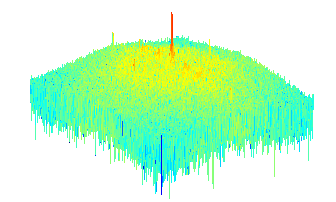
\includegraphics[width=0.23\textwidth]{figure-03a.png}}\hspace{1mm}
\subfloat[Attack video.]{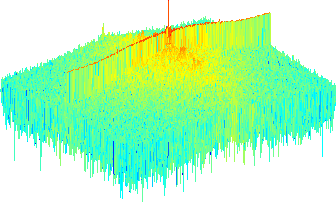
\includegraphics[width=0.23\textwidth]{figure-03b.png}}\\
\caption{\rv{Example of a video frame} of the spectra generated from (a) a valid video and (b) an attack video.}
\label{fig:spectrum}
\end{figure}

\subsection{Calculation of the Visual Rhythms}
In order to capture the temporal information contained in the Fourier Spectrum Videos ($\nu_{FS}$) and summarize their content, we employ the visual rhythm technique~\cite{Chung:KT:1999}. Visual rhythm is a simplification of a video content in a 2D image obtained by sampling regions of the video. Applications of this concept can be found in the work by Chun et al.~\cite{Chun:RAVIS:2002} that use visual rhythms for fast text caption localization on video, and Guimar\~{a}es et al.~ \cite{Guimaraes:SIBGRAPI:2001} who propose a method for gradual transition detection in videos. The use of visual rhythm in our work is crucial since it allows us to capture patterns that are present in the Fourier Spectrum Videos providing an effective way of viewing a video as \rv{a still image}. 

\rv{Considering a video $\nu$ in the $2D+t$ domain with $t$ frames of dimensions $W \times H$ pixels, the visual rhythm $I_{\nu_{R}}$ is a representation of the video $\nu$, in which regions of interest of each frame are sampled and aggregated to form a new image, called visual rhythm. The regions of interest must be carefully chosen to capture the patterns contained in $\nu_{FS}$. Formally, a visual rhythm $I_{\nu_{R}}$ of a video $\nu$ can be defined by 
%
\begin{eqnarray}
	I_{\nu_{R}}(z,t) = \nu(x(z),y(z), t),
\label{eq:rvformal}
\end{eqnarray}
\noindent where $x(z)$ and $y(z)$ are functions of the independent variable $z$. The visual rhythm is a two-dimensional image whose vertical $z$ axis consists of a certain group of pixels extracted from video $\nu$ and the samples are accumulated along the time $t$. Therefore, according to the mapping of $x(z)$ and $y(z)$, we can generate several types of visual rhythms~\cite{Chung:KT:1999}. For instance, the sampling of the central vertical pixels can be performed by applying $I_{\nu_{R}}(z,t) = \nu(x(\frac{W}{2}), y(z), t)$. Similarly, the central horizontal pixels can be extracted by applying \bmark{$I_{\nu_{R}}(z,t) = \nu(x(z), y(\frac{H}{2}), t)$.}}

Given that the lower responses are mainly concentrated at the abscissa and ordinate axes~\cite{Smith:SEG:1997} of the Fourier spectrum (see \rrv{Fig.}~\ref{fig:spectrum}), \rv{initially} we consider two regions of interest in the frames that form the spectrum video in the construction of two types of visual rhythms: (i) the horizontal visual rhythm formed by central horizontal lines and (ii) the vertical visual rhythm formed by central vertical lines. In both cases, we can summarize relevant content of the spectrum video in a single image. \rrv{Fig.}~\ref{fig:rv} depicts the visual rhythms generated by two regions of interest considering a valid (\rrv{Fig.}~\ref{fig:rv}(a) and~\ref{fig:rv}(c)) and an attack video (\rrv{Fig.}~\ref{fig:rv}(b)~and~\ref{fig:rv}(d)).
%
\begin{figure}[[!htb]
\centering
\subfloat[Valid video.]{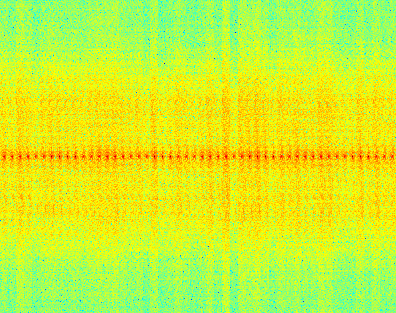
\includegraphics[width=0.16\textwidth]{figure-04a.png}}\hspace{1mm}
\subfloat[Attack video.]{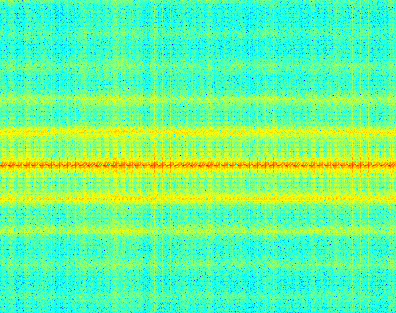
\includegraphics[width=0.16\textwidth]{figure-04b.png}}\\ 
\subfloat[Valid video.]{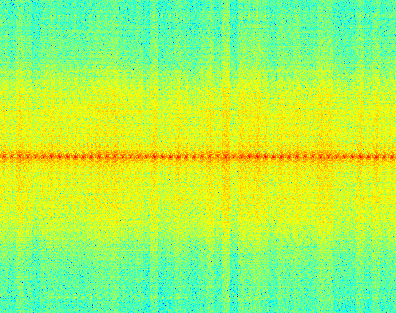
\includegraphics[width=0.16\textwidth]{figure-04c.png}}\hspace{1mm}
\subfloat[Attack video.]{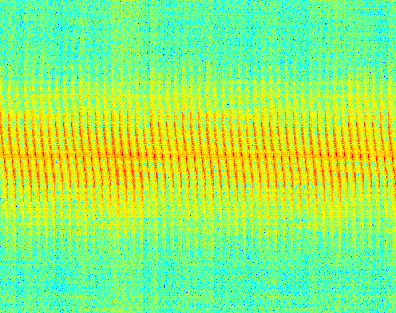
\includegraphics[width=0.16\textwidth]{figure-04d.png}}
\caption{\rv{Visual rhythms constructed} from (a)-(b) central horizontal lines and from (c)-(d) central vertical lines. Note that the visual rhythm obtained from horizontal lines has been rotated 90 degrees for {visualization purposes}.}
\label{fig:rv}
\end{figure}

Even though the visual rhythms are different for valid and attack videos, their construction disregards the highest responses that are not at the abscissa and ordinate axes and, in some cases, such information is important to make a better distinction between valid access and attempted attack videos, as shown in \rrv{Fig.}~\ref{fig:espectro}. With this in mind, we extract a third type of visual rhythm by traversing along the frames of Fourier Spectrum Videos ($\nu_{FS}$) in a zig-zag scheme. \rrv{Fig.}~\ref{fig:rvZigzag} shows the zig-zag visual rhythm generated for a valid access video and an attempted attack video.
%
\begin{figure}[!htb]
\centering
\subfloat[Valid video.]{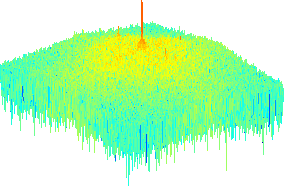
\includegraphics[width=0.2\textwidth]{figure-05a.png}}\hspace{1mm}
\subfloat[Attack video.]{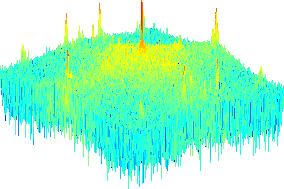
\includegraphics[width=0.2\textwidth]{figure-05b.png}}\\
\caption{Examples of spectra whose highest responses are not only at the abscissa and ordinates axes.}
\label{fig:espectro}
\end{figure}
%
\begin{figure}[!htb]
\centering
\subfloat[Valid video.]{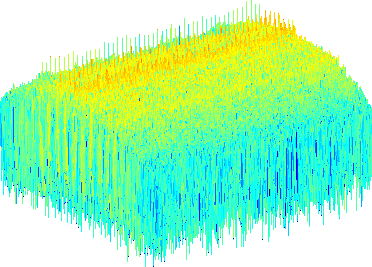
\includegraphics[width=0.2\textwidth]{figure-06a.png}}\hspace{1mm}
\subfloat[Attack video.]{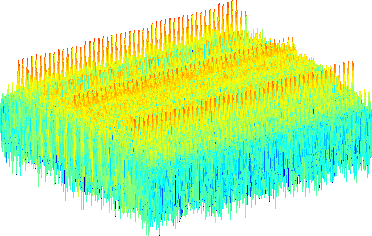
\includegraphics[width=0.2\textwidth]{figure-06b.png}}\\
\caption{Examples of visual rhythms constructed in a zig-zag traversal.}
\label{fig:rvZigzag}
\end{figure}

\subsection{Feature Extraction}
Once the visual rhythms are computed, we can use machine learning techniques to train a classifier to decide whether a biometric sample is fake or not. However, if the intensity of the pixels composing the visual rhythms are directly considered, the dimensionality of the feature space will be extremely high and most of the traditional classification methods will not work properly. Therefore, we need to extract a compact set of feature descriptors that best discriminate the visual rhythms generated from the fake and valid videos.

In this work, we evaluate the use of three feature descriptors: Gray Level Co-occurrence Matrices (GLCM)~\cite{Haralick:TSMC:1973}, Local Binary Patterns (LBP)~\cite{Ojala:TPAMI:2002} and \rv{Histogram of Oriented Gradients (HOG)}~\cite{Dalal:CVPR:2005}. \bmark{The choice for using GLCM and LBP descriptors is motivated by the fact that} the visual rhythms can be interpreted as texture maps (see \rrv{Fig.}~\ref{fig:rv}). Moreover, if we consider the intensity values of the pixels of the visual rhythms as height and edge artifacts represented along the maps, we see (\rrv{Fig.}~\ref{fig:rvZigzag}) that such images have \bmark{different edge forms, a property that can be reasonably explored} by the HOG descriptor.

\paragraph{GLCM}
It is a structure that describes the frequency of gray level occurrence between pairs of pixels. When normalized, the co-occurrence matrix becomes an estimation of joint probabilities between pairs of pixels at a distance $d$ in a given orientation $\theta$. After calculating the co-occurrence matrix for four different orientations, we extracted $12$ measures to summarize the textural information of each matrix: angular second-moment, contrast, correlation, variance, inverse difference moment, sum average, sum variance, sum entropy, entropy, difference variance, difference entropy, and directionality.

\paragraph{LBP}
{The LBP operator~\cite{Ojala:TPAMI:2002} provides a robust way to describe local binary patterns. \bmark{Basically, a window of size $3$} pixels is thresholded by the value of the central pixel. The pixel values are then multiplied by binomial weights and summed to obtain an LBP number to this window. Thus, LBP can produce up $2^{8} = 256$  different texture patterns, and a histogram with $256$ bins is calculated and used as a texture descriptor.}

\paragraph{HOG}
The basic idea of this descriptor relies on the fact that the local appearance of the objects and shape can be well characterized by the distribution of local intensity gradients or edge directions, even without precise knowledge of the corresponding gradient or edge positions. Basically, the image is divided into small spatial regions, \rv{referred to} as cells, and for each cell is calculated a histogram of gradient directions. A set of cells is grouped into a block and the concatenation of the descriptors extracted from each cell followed by a normalization results in the HOG descriptor.

\subsection{Learning}
We evaluate the proposed characterization process using two machine learning techniques: Support Vector Machine (SVM) and Partial Least Square (PLS) that are used in the construction of a binary classifier to decide whether a sample is fake or not. 

The SVM algorithm~\cite{Cortes:ML:1995} uses \rv{either a linear or a }non-linear mapping, depending on the type of space used to transform the original data onto a higher dimensional \rv{one}. %Within this new space, the SVM finds an optimal hyperplane that separates the input data into classes.

PLS regression method~\cite{Hoskuldsson_1988} is based on the linear transformation of a large number of descriptors to a new space based on a small number of orthogonal projection vectors. In other words, the projection vectors are mutually independent linear combinations of the original descriptors. These vectors are chosen to provide maximum correlation with the dependent variables, which are the labels of the training classes.

\section{Database Creation}
\label{sec:DatabaseCreation}

This section presents the Unicamp Video-Attack Database (UVAD) specifically built for evaluation of the video-based spoofing attack detection methods. The UVAD contains valid access and attempted attack videos of $404$ different identities. All videos were created at Full HD quality, with $30$ frames per second and \rv{are} nine seconds long.

The generation of valid access videos was performed by filming each participant in two sections considering different backgrounds, lighting conditions, and places (\rv{indoors and outdoors}). \bmark{As each person is recorded by only one camera, then there is no identity overlap between video from different camera.} In total, $808$ videos that represent valid \rv{accesses were generated with six different cameras: a $9.1$ megapixels Sony CyberShot DSC-HX1, a $10.0$ megapixels Canon PowerShot SX1 IS, a $10.3$ megapixels Nikon Coolpix P100, a $14.0$ megapixels Kodak Z981, a $14.0$ megapixels Olympus SP 800UZ, and a $12.1$ megapixels Panasonic FZ35 digital camera}. We used a tripod to avoid disturbance in the videos during the recordings. The generated videos were cropped to maintain a resolution of $1,366 \times 768$ and allow the faces to be positioned at the center of the video frame. No resampling was performed whatsoever.

\rv{The attempted attack videos were generated by using the same digital cameras utilized to generate the valid access videos and seven different display devices with a $1,366 \times 768$ pixel resolution. The valid access videos were displayed on seven display devices and {recaptured with the same digital cameras used previously}. Each display device was positioned in front of each camera at a distance of $90 \pm 5$cm supported in a tripod, so that to ensure each video with $1,366 \times 768$ resolution after cropping.}

As the valid access videos were cropped to maintain a $1,366 \times 768$ resolution, we guarantee that there was no scaling transformations during their exhibition. \rv{In total, we have generated $16,268$ attempted attack videos and $808$ valid access videos. Fig.~\ref{fig:exemplosVideosValidos} and~\ref{fig:exemplosVideosAtaque} depict real and fake video frame examples, respectively.}
%
\begin{figure*}[!htb]
\centering
\begin{tabular}{c}
	\includegraphics*[width=0.15\textwidth]{figure-07a.png}
	\includegraphics*[width=0.15\textwidth]{figure-07b.png}
	\includegraphics*[width=0.15\textwidth]{figure-07c.png}
	\includegraphics*[width=0.15\textwidth]{figure-07d.png}
	\includegraphics*[width=0.15\textwidth]{figure-07e.png}
\end{tabular}
\caption{Examples of valid access video frames for outdoor (first and second images on the left) and indoor (three images on the right) scenes.}
\label{fig:exemplosVideosValidos}
\end{figure*}
%
\begin{figure*}[!htb]
\centering

\begin{tabular}{c}
	\includegraphics*[width=0.15\textwidth]{figure-08a.png}
	\includegraphics*[width=0.15\textwidth]{figure-08b.png}
	\includegraphics*[width=0.15\textwidth, height=0.105\textheight]{figure-08c.png}
	\includegraphics*[width=0.15\textwidth, height=0.105\textheight]{figure-08d.png}
	\includegraphics*[width=0.15\textwidth, height=0.105\textheight]{figure-08e.png}

\end{tabular}
\caption{Examples of attempted attack video frames for outdoor (first and second images on the left) and indoor (three images on the right) scenes using Sony (first and second columns), Canon (third and fourth columns) and Nikon (last column) cameras.}
\label{fig:exemplosVideosAtaque}
\end{figure*}

%\rrv{Fig.}~\ref{fig:exemplosVideosValidos} illustrates real \rv{and fake video frames of UVAD dataset.}
%%
%\begin{figure*}[!htb]
%\centering
%\begin{tabular}{c}
%	\includegraphics*[width=0.18\textwidth]{facesReais/MAH00938.PNG}
%	\includegraphics*[width=0.18\textwidth]{facesReais/MAH01502.PNG}
%	\includegraphics*[width=0.18\textwidth]{facesFakes/MAH00938.PNG}
%	\includegraphics*[width=0.18\textwidth, height=0.105\textheight]{facesFakes/MAH01241.PNG}
%	\includegraphics*[width=0.18\textwidth, height=0.105\textheight]{facesFakes/MAH01502.PNG}	
%\end{tabular}
%\caption{Examples of valid access video frames (first and second images on the left) \rv{and attempted} attack video frames (last three columns) using different cameras for indoor and outdoor scenes.}
%\label{fig:exemplosVideosValidos}
%\end{figure*}

Table~\ref{table:database} shows a comparison between the proposed UVAD database and some other reference benchmarks in the literature. The diversity of display devices and acquisition sensors used in the generation of {UVAD} is an important characteristic that is not found in the other databases, which was essential to a better comprehension of the problem and for a precise evaluation of the \rv{methods as we will show in Section~\ref{sec:ExperimentsAndResults}.}

\begin{table*}[!htb]
\centering
\caption{Comparison of the proposed UVAD database and other available reference benchmarks in the literature.}
\label{table:database}
\begin{tabular}{llllll}
\toprule
\multirow{2}{*}{\textbf{Database}} & \textbf{Number of} & \textbf{Number of} & \textbf{Number of} & \textbf{Number of} & \textbf{Number of devices used} \\
             & \textbf{subjects} & \textbf{valid accesses} & \textbf{attacks by photo} & \textbf{attacks by video} & \textbf{to create the attack videos}\\
\otoprule
NUAA~\cite{Tan:ECCV:2010} & 15 & $ 5,105$ & $7,509$ & --- & ---\\
\cline{1-6}
Print-Attack~\cite{Anjos:IJCB:2011} & $50$ & $200$ & $200$ & --- & ---\\
\cline{1-6}

\multirow{1}{*}{CASIA~\cite{Zhang:ICB:2012}} & \multirow{1}{*}{$50$} & \multirow{1}{*}{$150$} & \multirow{1}{*}{$300$} & \multirow{1}{*}{$150$} & $3$ cameras and $1$ display device\\
%             &       &       &     &          & \\
\cline{1-6}

Replay-Attack~\cite{Chingovska:BIOSEG:2012} & $50$ & $200$ & $200$ & $800$ & $2$ cameras and $2$ display devices\\
%             &       &       &     &          & \\
\cline{1-6}

UVAD (proposed) & \rv{$404$} & \rv{$808$} & --- & \rv{$16,268$} & \rv{$6$ cameras and $7$ display devices}\\
%             &       &       &     &          & \\
\bottomrule
\end{tabular}
\end{table*}

\section{Experimental Results}
\label{sec:ExperimentsAndResults}
In this section, we show the details of the experiments and performance evaluations of the developed method. We \rv{first consider the UVAD database which was introduced} in Section~\ref{sec:DatabaseCreation} (Experiments I-IV). The diversity of \rv{devices used} allows us to answer important questions regarding some strengths and limitations of the proposed method. \rv{In addition, we also evaluate the proposed method with respect to the literature (Experiment~V) and through the Replay-Attack Database (c.f.,~Sec.~\ref{sec:replay:attack}) (Experiment VI).}

\subsection{Protocols for the UVAD Database}
In this section, we define appropriate protocols for each experiment.

\rv{ %
\vspace{0.1cm}
\noindent\textbf{Protocol I.}
The aim of this protocol is at finding the best configuration of the proposed method. In this protocol, we divide the dataset into two sets, hereintofore referred to as training and test sets. During partition, we guarantee that there is no overlap of data from the same capture and display devices between training and test sets, so that we have a proper comparison without experimental bias.

The valid access videos from six cameras were divided into two subsets, {\emph{A} and \emph{B}}. The valid access videos in set \emph{A} were again divided to form two sets of valid access videos: (i)~real training set, composed of videos generated by three cameras chosen arbitrarily (Sony, Canon, and Kodak) and (ii) real test set, composed of videos generated by the remaining three cameras (Nikon, Olympus, and Panasonic).

In sequence, the valid access videos in set \emph{B} were used to generate two sets of attempted attack videos: (i) the fake training set, in which videos in \emph{B} generated by the Sony, Canon, and Kodak cameras were displayed on three display devices and recaptured by the same three cameras, and (ii) the fake test set, whose videos in \emph{B} generated by the Nikon, Olympus, and Panasonic cameras were displayed on the remaining three display devices and recaptured by the same cameras.

\vspace{0.1cm}
\noindent\textbf{Protocol II.}
The aim of this protocol is at checking the influence of the biometric sensor on the proposed method. Similarly to the previous protocol, we divide the dataset into two sets, training and test sets. However, we create nine training and test sets, changing the cameras that compose such sets. Again, we guarantee that there is no overlap of data from the same cameras and display devices. Our goal with these partitions is to train a classifier with videos from three cameras and test it with the videos from other three cameras that never were used or seen by the classifier.

\vspace{0.1cm}
\noindent\textbf{Protocol III.}
The aim of this protocol is at checking the influence of the display devices over the detection method. In this protocol, we divide the videos from each camera into two sets, \emph{A} and \emph{B}. Set \emph{A} contains attempted attacks performed with three display devices and set \emph{B} comprises attempted attacks performed with the three complementary  display devices. The partition considering different display devices for both attack sets was carried out to avoid that a classifier takes biased conclusions regarding videos coming from devices already seen during the training step. The classification results are given in terms of mean of the results obtained in two rounds of experiments by using the set \emph{A} to train a classifier and \emph{B} to test it, and vice versa.
}

\subsection{Parameters for the Filtering Process, Visual Rhythm Analysis and Classification}
{To extract signal noise signature of the videos, as Equation~\ref{eq:ruido} shows}, we consider the use of spatial linear and non-linear filters: a Gaussian filter with~$\mu = 0$,~$\sigma = 2$, and size~$ 7 \times 7$ and a Median filter with size~$7 \times 7$, respectively. These parameters were obtained empirically {in~\cite{Pinto:SIBGRAPI:2012} on a different dataset}.

After calculating the noise signature using Equations~\ref{eq:dft} and~\ref{eq:spectrum}, we extract the visual rhythms {(horizontal and vertical)} of each video considering the first $50$ frames and a block of either $30$ columns (vertical) pixels or $30$ lines (horizontal). Since the visual vertical and horizontal rhythms of each video {carry} different temporal information, we evaluate the two types of visual rhythms along with their combinations. The horizontal visual rhythms {(H)} are in a dimensional space of $1,366 \times 1,500$-$d$ while the vertical visual rhythms {(V)} are in $768 \times 1,500$-$d$. To generate the zig-zag visual rhythms {(Z)}, we {also} consider the first $50$ frames of the Fourier {Spectrum transformed videos}. We extract block lines of $30$ pixels through the traversal of the frames, from left to right, top to bottom. Thus, we obtained visual rhythms that are in a dimensional space of $17,482 \times 1,500$-$d$.

The high dimensionality and large amount of visual rhythms prevent us from using pixel intensities {directly} as features. Therefore, we consider the visual rhythms as texture maps and calculate their texture patterns using different characterization methods. For instance, for the standard configuration, we considered the GLCM descriptor with directions $\theta \in \{0^{o}, 45^{o}, 90^{o}, 135^{o}\}$, distance $d = 1$ and $16$ bins. {Table~\ref{table:dimensaoGLCM} shows the dimensionality {information} of each feature.}
%
\begin{table}[!htb]
%\linethickness{1.5mm}
\centering
{%
\caption{Number of features (dimensions) using either the direct pixel intensities as features or the features extracted by image description methods.}
\label{table:dimensaoGLCM}
\begin{tabular}{lrrr}
\toprule
\multirow{2}{*}{\textbf{Name}} & \multicolumn{3}{c}{\centering \textbf{Descriptor Dimensionality}}\\
\cmidrule(r){2-4}
& \multicolumn{1}{c}{\textbf{V}} & \multicolumn{1}{c}{\textbf{H}} & \multicolumn{1}{c}{\textbf{Z}}\\
\otoprule
Pixel Intensity & $1,152,000$ & $2,049,000$ & $26,223,000$ \\
\hline
LBP & $256$ & $256$ & $256$ \\
\hline
GLCM & $48$ & $48$ & $48$ \\
\hline
HOG & $36$ & $36$ & $36$ \\
\bottomrule
\end{tabular}
}
\end{table}
In order to evaluate the robustness of the extracted features, we can use them to train a classifier and generate a model capable of distinguishing valid and attack videos, and test the model effectiveness. In this paper, we use two classification techniques: SVM and PLS. For SVM, we use the LibSVM~\cite{Chang:2011:TIST} implementation and we analyze the radial basis function kernel, whose parameters were found using {LibSVM's built-in} grid search algorithm. For PLS, we use the DetectorPLS method~\cite{schwartz09c} and we analyze different numbers of factors. The factors are latent variables that give us the best predictive power and they are extracted from a set of independent variables and are used to predict a set of dependent variables. {The interested reader may refer to~\cite{schwartz09c} for more details on factor choices in PLS.}

\subsection{Experiment I: Finding the Best Configuration}
\rv{The objective here is to find the best configuration of our method and to evaluate the classifiers, visual rhythm setups and filters through the analysis of variance to assess which of these parameters \bmark{present higher in} influence.} In addition, we evaluate other important feature characterization methods found in the literature, namely Local Binary Pattern Histogram (LBP) and Histogram of Oriented Gradient (HOG) descriptors. Although we have considered the visual rhythms as texture maps, \bmark{it is worth analyzing the use} of shape descriptors such as HOG as well. With this experiment, it is possible to discover whether considering the visual rhythms as texture maps is the best choice. \rv{We carried out these experiments using the \emph{Protocol I} and considering the sets of attacks with videos recaptured by all cameras.}

\rrv{After performing statistical analysis with ANOVA and Tukey's HSD (Honestly Significant Difference) test in the results shown in Table~\ref{table:best_config}, the following conclusions can be drawn:~(1)~GLCM descriptor performance is statistically different from its HOG and LBP counterparts, as shown in Fig.~\ref{fig:descriptorstats}. As it outperforms the other descriptors with statistical significance, we can conclude that GLCM was able to extract the most discriminative information from the visual rhythms as texture maps better than its counterparts; (2)~both Gaussian and Median filters used in this work to generate Noise Residual Videos ($\nu_{NR}$) \bmark{did not produce statistically different results} (figure now shown here); (3)~methods for building the visual rhythms did not present results with differences statistically significant (See Fig.~\ref{fig:visualrhythmstats}); and (4)~with respect to the classification algorithm used in this work, we do not find statistical differences between the use of the SVM and PLS algorithms (figure not shown here). It is noteworthy that both ANOVA and \bmark{TukeyHSD's} tests allow us to reject the hypothesis of equality between comparisons, but not accept the hypothesis that they are equal, in cases that no statistical differences were found. Therefore, the best configuration considered is the one using Median filter, Horizontal and Vertical visual rhythms combined, GLCM descriptor to extract texture information from visual rhythms, and the PLS classification algorithm.}
%
\begin{table}[!h]
\linethickness{1.5mm}
\centering
\rv{%
\caption{Results (AUC) of the experiment in which we find the best configuration of our method considering all possible setups.}
\label{table:best_config}
\begin{tabular}{llllll}
\toprule
 &  & \multicolumn{2}{c}{\centering \textbf{PLS}} & \multicolumn{2}{c}{\centering \textbf{SVM}}\\
\cmidrule(r){3-6}
 Desc. & V. Rhythms & 
\multicolumn{1}{c}{Gaussian} & \multicolumn{1}{c}{Median} & 
\multicolumn{1}{c}{Gaussian} & \multicolumn{1}{c}{Median} \\

\otoprule
\multirow{4}{*}{\textbf{GLCM}} 
& V &
$59.65$\% & $84.33$\% &
$68.57$\% & $74.86$\% \\ 
\cmidrule(r){2-6}
& H &
$76.27$\% & $86.29$\% &
$76.09$\% & $72.55$\% \\  
\cmidrule(r){2-6}
& V + H &
$77.74$\% & {$\mathbf{91.43}$\%} &
$74.90$\% & $65.28$\% \\  
\cmidrule(r){2-6}
& Z &
$90.92$\% & $80.23$\% &
$83.22$\% & $63.59$\% \\ 
\otoprule

\multirow{4}{*}{\textbf{LBP}}
& V &
$61.21$\% & $72.29$\% &
$56.06$\% & $65.95$\% \\ 
\cmidrule(r){2-6}
& H &
$62.75$\% & $63.55$\% &
$70.02$\% & $67.76$\% \\ 
\cmidrule(r){2-6}
& V + H &
$64.61$\% & $70.81$\% &
$70.97$\% & $73.44$\% \\ 
\cmidrule(r){2-6}
& Z &
$67.44$\% & $55.70$\% &
$64.65$\% & $57.36$\% \\ 
\otoprule

\multirow{4}{*}{\textbf{HOG}}
& V &
$68.75$\% & $54.68$\% &
$67.86$\% & $67.90$\% \\ 
\cmidrule(r){2-6}
& H &
$54.68$\% & $64.76$\% &
$50.61$\% & $66.88$\% \\ 
\cmidrule(r){2-6}
& V + H &
$57.73$\% & $73.72$\% &
$66.96$\% & $73.54$\% \\
\cmidrule(r){2-6}
& Z &
$65.54$\% & $65.54$\% &
$52.35$\% & $52.35$\% \\
\bottomrule
\end{tabular}
}
\end{table}
\begin{figure}[!h]
\centering
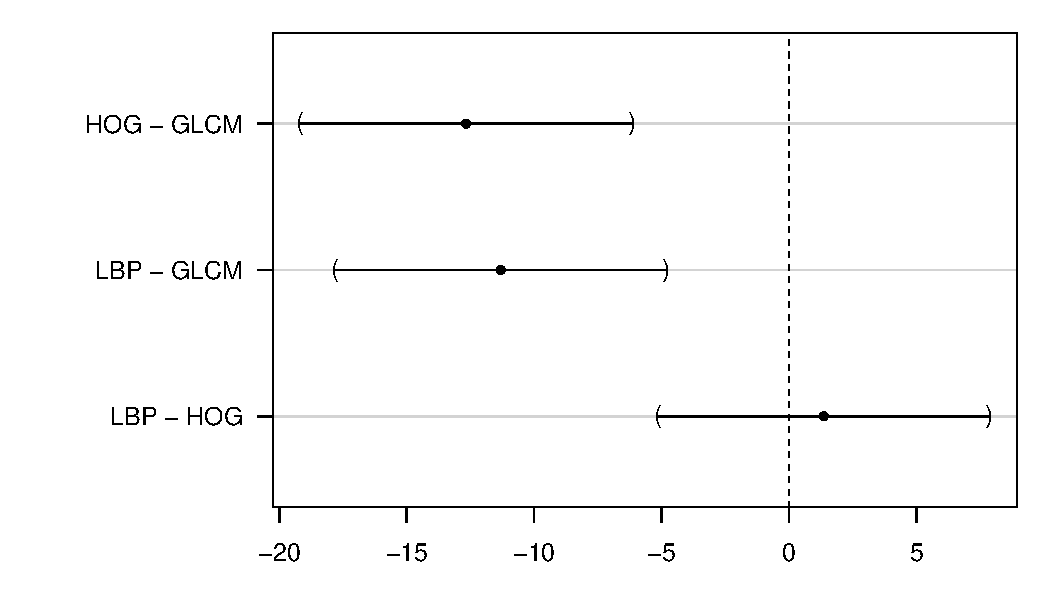
\includegraphics[width=0.32\textwidth]{figure-09.pdf}\\
\caption{{Differences in mean levels of the results obtained by the different descriptors used in this work and their confidence intervals for $95\%$ family-wise confidence level. There are statistical difference between the comparisons whose confidence intervals do not include zero.}}
\label{fig:descriptorstats}
\end{figure}
%
\begin{figure}[!h]
\centering
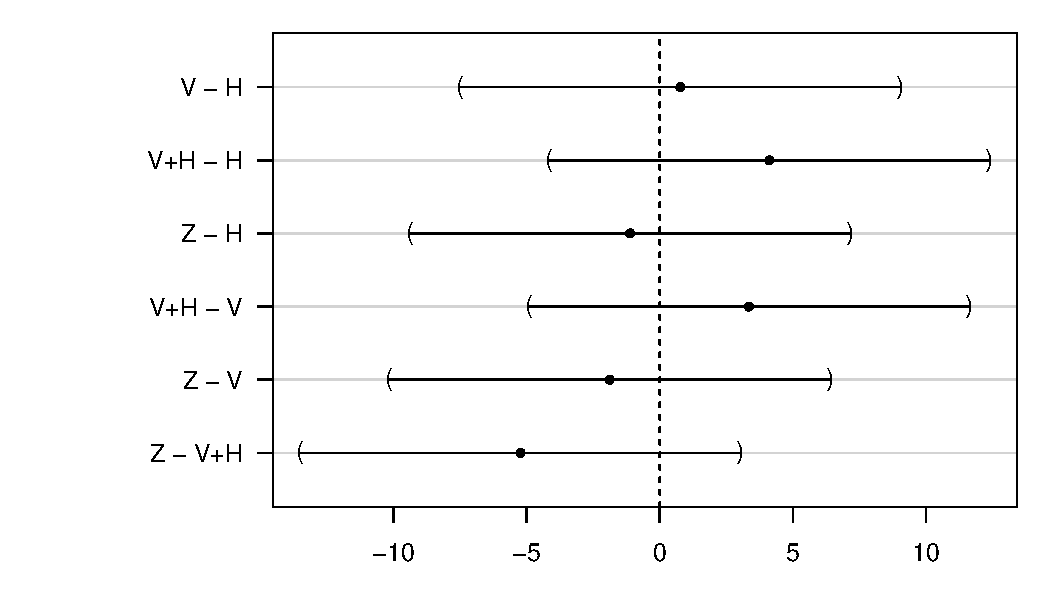
\includegraphics[width=0.32\textwidth]{figure-10.pdf}\\
\caption{{Differences in mean levels of the results obtained by the visual rhythms considered in this work and their confidence intervals for $95\%$ family-wise confidence level. There are statistical difference between the comparisons whose confidence intervals do not include zero.}}
\label{fig:visualrhythmstats}
\end{figure}
%
%\begin{figure}[!h]
%\centering
%\includegraphics[width=0.45\textwidth]{filter.pdf}\\
%\caption{{Differences in mean levels of the results obtained by the filters considered in this work and their confidence intervals for $95\%$ family-wise confidence level. There are statistical difference between the comparisons whose confidence intervals do not include zero.}}
%\label{fig:filter}
%\end{figure}
%
%\begin{figure}[!h]
%\centering
%\includegraphics[width=0.45\textwidth]{classifier.pdf}\\
%\caption{Differences in mean levels of the results obtained by the classifiers considered in this work and their confidence intervals for $95\%$ family-wise confidence level. There are statistical difference between the comparisons whose confidence intervals do not include zero.}
%\label{fig:classifier}
%\end{figure}

\subsection{Experiment II: Influence of the Biometric Sensors}
This experiment aims at checking whether the presented method works well in different facial biometric systems (biometric sensors). Experiments performed with only one kind of biometric sensor does not guarantee a broad evaluation of our method. \rv{Although this is not a common practice in the literature, we believe that experiments with several biometric sensors is an essential practice to evaluate countermeasure methods, because the artifact levels inserted into the biometric samples depend, among other factors, on the quality of the acquisition sensor. Using the~\emph{Protocol II}, we evaluate the proposed method in its best configuration (see Table~\ref{table:experimento2_median_pls}).}
%
\begin{table*}[!htb]
\centering
\rv{%
\caption{Results (AUC) of the experiment analyzing the influence of the biometric sensors using a PLS Classifier and Median Filter.}
\label{table:experimento2_median_pls}
\begin{tabular}{cccccccccc}
\toprule
\multirow{3}{*}{\textbf{Training}} 
&  Sony & Sony      & Sony    & Sony      & Sony    & Sony      & Canon     & Canon   & Canon \\
& Canon & Canon     & Canon   & Kodak     & Kodak   & Olympus   & Olympus   & Olympus & Kodak \\
& Kodak & Panasonic & Olympus & Panasonic & Olympus & Panasonic & Panasonic & Kodak   & Panasonic \\
\otoprule
\multirow{3}{*}{\textbf{Test}}
& Nikon     & Nikon   & Nikon    & Nikon   & Nikon     & Canon  & Sony   & Sony      & Sony \\
& Olympus   & Olympus & Kodak    & Canon   & Canon     & Kodak  & Kodak  & Nikon     & Nikon \\
& Panasonic & Kodak  & Panasonic & Olympus & Panasonic & Nikon  & Nikon  & Panasonic & Olympus \\

\otoprule
AUC & $91.43\%$ & $90.48\%$ & $86.89\%$ &$89.66\%$ & $96.12\%$ & $91.85\%$ & $81.07\%$ & $86.84\%$ & $84.25\%$ \\
\bottomrule
\end{tabular}
}
\end{table*}

\rv{When we vary the cameras used in the training, we have a variation in the method generalization. For instance, considering the best and worst results shown in the Table~\ref{table:experimento2_median_pls}, we have a relative error reduction of $79.50\%$. \bmark{Though it is evident the in} influence of the biometric sensor with this variation in the classification results, we performed the Wilcoxon Signed Rank test to prove this influence, with which we obtained a $p$-value of $0.0039$ and hence confirmation that the values shown in Table~\ref{table:experimento2_median_pls} are indeed statistically different.}

\subsection{Experiment III: Influence of the Display Devices}
\rv{\bmark{The aim of this experiment is to check} whether the presented method is able to detect attacks with different display devices, that is, whether the display devices produce different amounts of display artifacts (the main artifacts produced are flickering, mooring and banding effect).} This is an important question to be answered because if the method is not robust to different devices, learning techniques considering an open scenario could be considered~\cite{Scheirer:TPAMI:2012}, given that in this case the classifier should be able to recognize attacks with display devices for which it has no prior knowledge.

\rv{Considering \emph{Protocol III}, this experiment was performed in two rounds: firstly, we train a classifier with attacks performed with three display devices and tested it with the other three display devices to evaluate the model found by the classifier. Secondly, we switch the sets and redo the analysis. In both cases, we considered the best configuration of our method. The results reported in Table~\ref{table:experimento3} correspond to the average ($\overline{x}$) and stdev ($s$) of the results obtained in the two rounds for each configuration of the method.}
%
\begin{table*}[!htb]
\centering
\rv{%
\caption{Results (AUC) of the experiment analyzing the influence of the display devices using a PLS Classifier and Median Filter.}
\label{table:experimento3}
\begin{tabular}{cccccc}
\toprule
%\textbf{Visual Rhythms} & \multicolumn{3}{c}{\centering \textbf{PLS classifier and Median filter}}\\
%\cline{2-4}
\textbf{Sony} & \textbf{Canon} & \textbf{Nikon}& \textbf{Kodak}& \textbf{Olympus}& \textbf{Panasonic}\\
\otoprule
\tickYes  & \tickNo & \tickNo & \tickYes & \tickNo & \tickYes \\

\cline{1-6}
\textit{p--value} = $0.0$ & \textit{p--value} = $1.0$ & \textit{p--value} = $1.0$ & \textit{p--value} = $0.0$ & \textit{p--value} = $0.574$ & \textit{p--value} = $0.015$ \\
\cline{1-6}
$\overline{x}=92.70\%$ & $\overline{x}=99.34\%$ & $\overline{x}=98.61\%$ & $\overline{x}=96.42\%$ & $\overline{x}=84.57\%$ & $\overline{x}=97.53\%$\\
\cline{1-6}
$s=0.23\%$        & $s=0.91\%$         & $s=1.36\%$ & $s=0.76\%$        & $s=14.33\%$         & $s=2.81\%$\\
\bottomrule

\end{tabular}
}
\end{table*}

\rv{The influence of the display devices are evidenced when the results obtained in the two rounds of experiments are discrepant or whether they are statistically different, indicating that the method was not able to detect attempted attacks performed with unknown display devices. To verify whether the differences in the results are statistically significant, we carried out a hypothesis test for two unpaired or independent samples. Once the sample values are nominal, the most appropriate statistical test is $\chi^{2}$ test for two samples whose values are also shown in all tables, considering a confidence level of $95$\%. The $p$-value produced for the $\chi^{2}$ tests evaluate whether two samples are statistically different ($p$-value $<$ $0.05$). According to results shown in Table~\ref{table:experimento3}, we have obtained a $p$-value lower than $\alpha = 0.05$, for some cameras. In these cases, the differences were statistically significant, which leads us to the conclusion that the display device plays an important role in the spoofing detection task.}

\subsection{Experiment IV: Comparison to a State-of-the-Art Method for Photo-Based Spoofing Attack Detection}
In the final round of experiments concerning the UVAD database, we compare our method to the one proposed in~\cite{Schwartz:IJCB:2011}. We considered the \emph{Protocol I} to compare both methods. It was not possible to run the algorithm by Schwartz et al. by using the same parameters described in~\cite{Schwartz:IJCB:2011} due to the high dimensionality of the data {their method produces}, even on a machine with $48$GB of RAM. The dimensionality of the feature vector generated by the original algorithm is higher than five million dimensions for each video frame.

In order to reduce the dimensionality of the feature vectors, we applied the HOG descriptor \rv{with blocks of sizes $16 \times 16$ and $32\times 32$ with strides of $16$ and $32$ pixels, respectively. The other parameters were set as described in~\cite{Schwartz:IJCB:2011}. With this, we were able to reduce the feature vector dimensionality to $8,880$ dimensions.} Table~\ref{table:comparacao_ijcb} shows the results obtained by using the algorithm in~\cite{Schwartz:IJCB:2011} and our method, considering the configuration that yielded the lowest classification error. \rv{Furthermore, the computational time spent by the algorithm in~\cite{Schwartz:IJCB:2011} was $\approx 237$ hours to process all the data, whereas the method proposed in this work spent $\approx 72$ hours. \bmark{According to McNemar statistical test, the result obtained by the methods are statistically different.}} All experiments were conducted on an Intel Xeon E$5620$, $2.4$GHz quad core processor with $48$GB of RAM under Linux operating system.

With this experiment, we can conclude that our method better characterized video-based attacks while being more efficient and suitable for different classification techniques, once it provides more compact feature representations.

\begin{table}[h]
\centering
\rv{%
\caption{Comparison between~\cite{Schwartz:IJCB:2011} and the method proposed in this work in its best setup (using combined visual rhythm, Median filter and a PLS Classifier).}
\label{table:comparacao_ijcb}
\begin{tabular}{cl}
\toprule
% & \multicolumn{4}{c}{\centering \textbf{PLS classifier and Median filter}}\\
%\otoprule
 & AUC (\%)\\
\otoprule
Schwartz et al.~\cite{Schwartz:IJCB:2011} & $90.52\%$ \\ 
\cline{1-2}
Our method & $\textbf{91.43}\%$ \\
\otoprule
Error Reduction & $9.60\%$ \\
\bottomrule
\end{tabular}
}
\end{table}

\subsection{Experiment V: Evaluation of the Method in the Replay-Attack Database}
In this experiment, we evaluate our method on the Replay-Attack database (c.f.,~\ref{sec:replay:attack}) which contains photo-based and video-based spoofing attacks. The goal of this experiment is to verify the effectiveness of our method on these several types of attacks. We use the experimental protocol described in~\cite{Chingovska:BIOSEG:2012}, whose results are shown in Table~\ref{table:replayEval}. Although our \bmark{method is designed for video-based spoofing attack detection}, we have obtained a promising AUC of $\approx 93\%$. For reference, in~\cite{Chingovska:BIOSEG:2012}, \bmark{the authors reported a Half Total Error Rate (HTER) of $34.01\%$ and $15.16\%$, using a $\chi^{2}$ and SVM classifier, respectively, to classify LBP$_{3\times2}^{u2}$ features,} while our method yields an HTER of $14.27\%$. We use a Gaussian filter with $\mu = 0$, $\sigma = 0.5$ and size $3 \times 3$, and a Median filter with size $3 \times 3$. These parameters were empirically obtained by using the Replay-Attack Database. With this experiment, we can conclude that the proposed method is able not only to detect video-based spoof attacks but also video print-attacks.

Finally, one can notice that, in particular, the zig-zag characterization method does not lead to the best result in this dataset. We believe the reason is that the Replay-Attack~\cite{Chingovska:BIOSEG:2012} is a dataset based on print photograph recaptures (still image attacks) which, when recaptured, tend to concentrate visual information in the center of the Fourier transformed domain as depicted in \rrv{Fig.}~\ref{fig:spectrum_datasets:replay}. This tends to favor the vertical and horizontal visual rhythms as they concentrate on these areas. The contrary happens with video attacks since the peaks in the Fourier transformed domain will be more spatially spread over each frame, as shown in \rrv{Fig.}~\ref{fig:espectro}. \bmark{Result obtained by the TukeyHSD' test confirm that difference between V+H and Z visual rhythms are statistically significant (p-value=$0.03$).}
%
\begin{table}[!htb]
\caption{Results (AUC) for the test set of the Replay-Attack database}
\label{table:replayEval}
\centering
\begin{tabular}{cllll}
\toprule
\multirow{2}{*}{Visual Rhythms} & \multicolumn{2}{c}{\centering \textbf{PLS classifier}} & \multicolumn{2}{c}{\centering \textbf{SVM classifier}}\\
\cline{2-5}
     & \textbf{Median} & \textbf{Gaussian} & \textbf{Median} & \textbf{Gaussian}\\
\otoprule
V & $83.99\%$ & $89.01\%$ & $86.26\%$ & $91.56\%$ \\ 
\hline
H & $81.98\%$ & $85.66\%$ & $80.67\%$ & $73.36\%$ \\ 
\hline
V + H & $90.69\%$ & $92.98\%$ & $92.01\%$ & $91.81\%$ \\ 
\hline
Z & $78.39\%$ & $85.35\%$ & $86.56\%$ & $77.72\%$ \\ 
\bottomrule
\end{tabular}
\end{table}
%
\begin{figure}[htb]
\centering
\subfloat[ ]{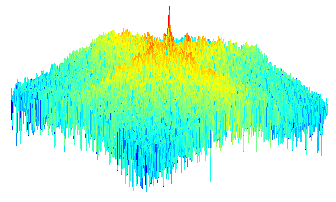
\includegraphics[width=0.23\textwidth]{figure-11a.png}} 
\subfloat[ ]{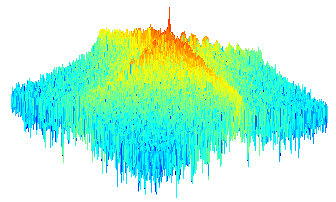
\includegraphics[width=0.23\textwidth]{figure-11b.png}} \\
%\subfloat[ ]{\includegraphics[width=0.23\textwidth]{espectroUvad1.png}} \hspace{1mm}
%\subfloat[ ]{\includegraphics[width=0.23\textwidth]{espectroUvad2.png}} \\
\caption{{Example of a video frame of the spectra generated from (a) a valid access video of the Replay-Attack database and (b) a video of an attempted attack of the same dataset. Note a concentration of information on the center rather than spread over as for the videos case shown in~\rrv{Fig.}~\ref{fig:espectro}.}}
\label{fig:spectrum_datasets:replay}
\end{figure}
%
%\begin{figure}
%\centering
%\includegraphics[width=0.6\linewidth]{./figures/replay_attack_stats}
%\caption{Differences in mean levels of the results obtained, using the Replay-Attack Database,  by the visual rhythms considered in this work and their confidence intervals for 95\% family-wise confidence level. There are statistical difference between the comparisons whose confidence intervals do not include zero.}
%\label{fig:replay_attack_stats}
%\end{figure}
%
%


%IJCB method = 237h
%our method = 2877s +

\section{Conclusions and Future Work}
\label{sec:Conclusion}

\bmark{Biometric authentication systems have been shown to be vulnerable} to spoofing attacks in the sense that impostors can gain access privileges to resources as valid users. Spoofing attacks to a face recognition system can be performed by presenting it a photograph, a video, or a face mask of a legitimate user.

This paper proposed and evaluated a spatio-temporal method for video-based face spoofing detection through the analysis of noise signatures generated by the video acquisition process, which can be used to distinguish between valid and fake access videos. Noise properties are captured using Fourier spectrum for each frame of the video. \rv{A compact representation, called visual rhythm, is employed to detect temporal information in the Fourier spectrum. \bmark{Three different video traversal strategies were considered to form the visual rhythms, of which horizontal and vertical combined was shown to be the most effective.} Features were extracted from the visual rhythms through GLCM, LBP and HOG descriptors to allow a proper distinction between fake and real biometric data. \bmark{The GLCM method was shown to be the most discriminative and compact feature representation for visual rhythm description.}} 

\rv{An extensive data set, containing real access and spoofing attack videos, was created to evaluate the proposed method, as well as the state-of-the-art approaches. Through the conducted experiments, it is possible to conclude that the display devices and biometric sensors play an important role in the spoofing detection task. \rv{These findings are very important in making the future anti-spoofing methods more effective and guiding the development of new databases which must be more realistic, as the UVAD Database proposed in this paper.} The proposed anti-spoofing method provided competitive or even superior results in the tests when compared to state-of-the-art approaches.}

Although this paper represents a step toward solving the spoofing problem, it makes it clear that the problem is not fully-solved yet and poses new questions on future methods regarding how to better handle and tackle \rv{with new attacks due to the ever-growing market of acquisition and display devices such as hight quality monitors, hand-held and smartphone devices.} \rv{In this sense, the dataset provided in this paper will be available at the IEEE Information Forensics and Security Technical Committee website (\underline{{\url{http://tinyurl.com/pas4t9r}}}) and also registered with a proper DOI through FigShare (\underline{\url{http://figshare.com/}}) \bmark{in order to advance the frontier of research in spoofing detection.}}

Future research efforts branch out into devising other spatio-temporal descriptors that capture motion telltales associated with the recapture process as well as verifying other \rv{liveness detection problems other than face recognition such as video recapturing, piracy detection, among others~\cite{Bestagini:2013}}. 


\section*{Acknowledgments}
We thank the support of CAPES through the DeepEyes project, CNPq (\#304352/2012-8 and \#477662/2013-7), FAPESP (\#2010/05647-4 and \#2011/22749-8), FAPEMIG and Microsoft for the support.


\ifCLASSOPTIONcaptionsoff
  \newpage
\fi


\bibliographystyle{IEEEtran}
%\bibliography{References}
\begin{thebibliography}{10}
\providecommand{\url}[1]{#1}
\csname url@samestyle\endcsname
\providecommand{\newblock}{\relax}
\providecommand{\bibinfo}[2]{#2}
\providecommand{\BIBentrySTDinterwordspacing}{\spaceskip=0pt\relax}
\providecommand{\BIBentryALTinterwordstretchfactor}{4}
\providecommand{\BIBentryALTinterwordspacing}{\spaceskip=\fontdimen2\font plus
\BIBentryALTinterwordstretchfactor\fontdimen3\font minus
  \fontdimen4\font\relax}
\providecommand{\BIBforeignlanguage}[2]{{%
\expandafter\ifx\csname l@#1\endcsname\relax
\typeout{** WARNING: IEEEtran.bst: No hyphenation pattern has been}%
\typeout{** loaded for the language `#1'. Using the pattern for}%
\typeout{** the default language instead.}%
\else
\language=\csname l@#1\endcsname
\fi
#2}}
\providecommand{\BIBdecl}{\relax}
\BIBdecl

\bibitem{Jain:HB:2008}
A.~K. Jain and A.~Ross, \emph{{Handbook of Biometrics}}.\hskip 1em plus 0.5em
  minus 0.4em\relax Springer, 2008, ch. Introduction to Biometrics, pp. 1--22.

\bibitem{Buhan:CTITUT:2005}
I.~R. {Buhan} and P.~H. {Hartel}, ``The state of the art in abuse of
  biometrics,'' Centre for Telematics and Information Technology University of
  Twente, Enschede, Technical Report TR-CTIT-05-41, September 2005.

\bibitem{Tan:ECCV:2010}
X.~Tan, Y.~Li, J.~Liu, and L.~Jiang, ``Face liveness detection from a single
  image with sparse low rank bilinear discriminative model,'' in \emph{European
  Conference on Computer Vision}, 2010, pp. 504--517.

\bibitem{Maatta:IJCB:2011}
J.~M\"{a}\"{a}tt\"{a}, A.~Hadid, and M.~Pietik\"{a}inen, ``Face spoofing
  detection from single images using micro-texture analysis,'' in \emph{Intl.
  Joint Conference on Biometrics}, oct. 2011, pp. 1 --7.

\bibitem{Schwartz:IJCB:2011}
W.~Robson~Schwartz, A.~Rocha, and H.~Pedrini, ``Face spoofing detection through
  partial least squares and low-level descriptors,'' in \emph{Intl. Joint
  Conference on Biometrics}, oct. 2011, pp. 1 --8.

\bibitem{Pan:ICCV:2007}
G.~Pan, L.~Sun, Z.~Wu, and S.~Lao, ``Eyeblink-based anti-spoofing in face
  recognition from a generic webcamera,'' in \emph{IEEE Intl. Conference on
  Computer Vision}, oct. 2007, pp. 1 --8.

\bibitem{Li:ICMLC:2008}
J.-W. Li, ``Eye blink detection based on multiple gabor response waves,'' in
  \emph{IEEE Intl. Conference on Machine Learning and Cybernetics}, vol.~5,
  july 2008, pp. 2852 --2856.

\bibitem{Xu:ICIP:2008}
C.~Xu, Y.~Zheng, and Z.~Wang, ``Eye states detection by boosting local binary
  pattern histogram features,'' in \emph{IEEE Intl. Conference on Image
  Processing}, oct. 2008, pp. 1480--1483.

\bibitem{Pan:TS:2011}
G.~Pan, L.~Sun, Z.~Wu, and Y.~Wang, ``\BIBforeignlanguage{English}{Monocular
  camera-based face liveness detection by combining eyeblink and scene
  context},'' \emph{\BIBforeignlanguage{English}{Telecommunication Systems}},
  vol.~47, pp. 215--225, 2011.

\bibitem{Anjos:IJCB:2011}
A.~Anjos and S.~Marcel, ``Counter-measures to photo attacks in face
  recognition: A public database and a baseline,'' in \emph{Intl. Joint
  Conference on Biometrics}, oct. 2011, pp. 1 --7.

\bibitem{Pinto:SIBGRAPI:2012}
A.~Pinto, H.~Pedrini, W.~R. Schwartz, and A.~Rocha, ``Video-based face spoofing
  detection through visual rhythm analysis,'' in \emph{Conference on Graphics,
  Patterns and Images}, Ouro Preto, MG, Brazil, august 2012, pp. 221--228.

\bibitem{Pan_2008}
G.~Pan, Z.~Wu, and L.~Sun, \emph{Recent Advances in Face Recognition}.\hskip
  1em plus 0.5em minus 0.4em\relax InTech, 2008, ch. Liveness detection for
  face recognition, pp. 235--252.

\bibitem{Zhang:ICB:2012}
Z.~Zhang, J.~Yan, S.~Liu, Z.~Lei, D.~Yi, and S.~Li, ``A face antispoofing
  database with diverse attacks,'' in \emph{IAPR Intl. Conference on
  Biometrics}, 29 2012-april 1 2012, pp. 26 --31.

\bibitem{Chingovska:BIOSEG:2012}
I.~Chingovska, A.~Anjos, and S.~Marcel, ``On the effectiveness of local binary
  patterns in face anti-spoofing,'' in \emph{Intl. Conference of the Biometrics
  Special Interest Group}, sept. 2012, pp. 1 --7.

\bibitem{Tronci:IJCB:2011}
R.~Tronci, D.~Muntoni, G.~Fadda, M.~Pili, N.~Sirena, G.~Murgia, M.~Ristori, and
  F.~Roli, ``Fusion of multiple clues for photo-attack detection in face
  recognition systems,'' in \emph{Intl. Joint Conference on Biometrics}, oct.
  2011, pp. 1 --6.

\bibitem{Yan:ICARCV:2012}
J.~Yan, Z.~Zhang, Z.~Lei, D.~Yi, and S.~Z. Li, ``Face liveness detection by
  exploring multiple scenic clues,'' in \emph{IEE Intl. Conference on Control
  Automation Robotics and Vision}, dec 2012.

\bibitem{Li:BTHI:2004}
J.~Li, Y.~Wang, T.~Tan, and A.~K. Jain, ``Live face detection based on the
  analysis of fourier spectra,'' in \emph{Biometric Technology for Human
  Identification}, 2004, pp. 296--303.

\bibitem{Peixoto:ICIP:2011}
B.~Peixoto, C.~Michelassi, and A.~Rocha, ``Face liveness detection under bad
  illumination conditions,'' in \emph{IEEE Intl. Conference on Image
  Processing}, sept. 2011, pp. 3557 --3560.

\bibitem{Maatta:IET:2012}
J.~Maatta, A.~Hadid, and M.~Pietikainen, ``Face spoofing detection from single
  images using texture and local shape analysis,'' \emph{IET Biometrics},
  vol.~1, no.~1, pp. 3 --10, march 2012.

\bibitem{Kim:ICB:2012}
G.~Kim, S.~Eum, J.~K. Suhr, D.~I. Kim, K.~R. Park, and J.~Kim, ``Face liveness
  detection based on texture and frequency analyses,'' in \emph{IAPR Intl.
  Conference on Biometrics}, 29 2012-april 1 2012, pp. 67 --72.

\bibitem{Bao:ICIASP:2009}
W.~Bao, H.~Li, N.~Li, and W.~Jiang, ``A liveness detection method for face
  recognition based on optical flow field,'' in \emph{IEEE Intl. Conference on
  Image Analysis and Signal Processing}, april 2009, pp. 233--236.

\bibitem{Kollreider:IVC:2009}
K.~Kollreider, H.~Fronthaler, and J.~Bigun, ``Non-intrusive liveness detection
  by face images,'' \emph{Image and Vision Computing}, vol.~27, no.~3, pp.
  233--244, 2009.

\bibitem{Marsico:ICB:2012}
M.~De~Marsico, M.~Nappi, D.~Riccio, and J.~Dugelay, ``Moving face spoofing
  detection via 3d projective invariants,'' in \emph{IAPR Intl. Conference on
  Biometrics}, 29 2012-april 1 2012, pp. 73 --78.

\bibitem{Biggio:IJCB:2011}
B.~Biggio, Z.~Akthar, G.~Fumera, G.~Marcialis, and F.~Roli, ``Robustness of
  multi-modal biometric verification systems under realistic spoofing
  attacks,'' in \emph{IEEE Intl. Conference on Biometrics: Theory Applications
  and Systems}, oct. 2011, pp. 1 --6.

\bibitem{Marasco:ICMCS:2011}
E.~Marasco, P.~Johnson, C.~Sansone, and S.~Schuckers, ``Increase the security
  of multibiometric systems by incorporating a spoofing detection algorithm in
  the fusion mechanism,'' in \emph{Intl. Conference on Multiple Classifier
  Systems}, 2011, pp. 309--318.

\bibitem{Akhtar:ICIAP:2011}
Z.~Akhtar, G.~Fumera, G.~L. Marcialis, and F.~Roli, ``Robustness evaluation of
  biometric systems under spoof attacks,'' in \emph{Intl. Conference on Image
  Analysis and Processing}, 2011, pp. 159--168.

\bibitem{Akhtar:BTAS:2012}
------, ``Evaluation of serial and parallel multibiometric systems under
  spoofing attacks,'' in \emph{IEEE Intl. Conference on Biometrics: Theory
  Applications and Systems}, sept. 2012, pp. 283 --288.

\bibitem{Biggio:IET:2012}
B.~Biggio, Z.~Akhtar, G.~Fumera, G.~Marcialis, and F.~Roli, ``Security
  evaluation of biometric authentication systems under real spoofing attacks,''
  \emph{IET Biometrics}, vol.~1, no.~1, pp. 11 --24, march 2012.

\bibitem{Lukas:TIFS:2006}
J.~Luk\"{a}s, J.~Fridrich, and M.~Goljan, ``Digital camera identification from
  sensor pattern noise,'' \emph{IEEE Trans. on Information Forensics and
  Security}, vol.~1, no.~2, pp. 205 -- 214, june 2006.

\bibitem{Rocha:CSUR:2011}
A.~Rocha, W.~Scheirer, T.~Boult, and S.~Goldenstein, ``Vision of the unseen:
  Current trends and challenges in digital image and video forensics,''
  \emph{ACM Comput. Surv.}, vol.~43, no.~4, pp. 26:1--26:42, Oct. 2011.

\bibitem{Beach:PP:2008}
A.~Beach, \emph{Real world video compression}, 1st~ed.\hskip 1em plus 0.5em
  minus 0.4em\relax Berkeley, CA, USA: Peachpit Press, 2008.

\bibitem{Chung:KT:1999}
M.-G. Chung, J.~Lee, H.~Kim, S.~M.-H. Song, and W.-M. Kim, ``{Automatic Video
  Segmentation based on Spatio-Temporal Features},'' \emph{Korea Telecom},
  vol.~1, no.~4, pp. 4--14, 1999.

\bibitem{Chun:RAVIS:2002}
S.~S. Chun, H.~Kim, K.~Jung-Rim, S.~Oh, and S.~Sull, ``{Fast Text Caption
  Localization on Video Using Visual Rhythm},'' in \emph{Recent Advances in
  Visual Information Systems}, ser. Lecture Notes in Computer Science, S.-K.
  Chang, Z.~Chen, and S.-Y. Lee, Eds., 2002, vol. 2314, pp. 43--58.

\bibitem{Guimaraes:SIBGRAPI:2001}
S.~J.~F. Guimaraes, M.~Couprie, N.~J. Leite, and A.~A. Araujo, ``{A Method for
  Cut Detection Based on Visual Rhythm},'' in \emph{Conference on Graphics,
  Patterns and Images}, 2001, pp. 297--304.

\bibitem{Smith:SEG:1997}
S.~W. Smith, \emph{{The Scientist and Engineer's Guide to Digital Signal
  Processing}}.\hskip 1em plus 0.5em minus 0.4em\relax San Diego, CA, USA:
  California Technical Pub., 1997.

\bibitem{Haralick:TSMC:1973}
R.~M. Haralick, K.~Shanmugam, and I.~Dinstein, ``Textural features for image
  classification,'' \emph{IEEE Trans. on Systems, Man, and Cybernetics}, vol.
  SMC-3, no.~6, pp. 610 --621, nov. 1973.

\bibitem{Ojala:TPAMI:2002}
T.~Ojala, M.~Pietikainen, and T.~Maenpaa, ``Multiresolution gray-scale and
  rotation invariant texture classification with local binary patterns,''
  \emph{IEEE Trans. on Pattern Analysis and Machine Intelligence}, vol.~24,
  no.~7, pp. 971 --987, jul 2002.

\bibitem{Dalal:CVPR:2005}
N.~Dalal and B.~Triggs, ``Histograms of oriented gradients for human
  detection,'' in \emph{IEEE Intl. Conference on Computer Vision and Pattern
  Recognition}, vol.~1, june 2005, pp. 886 --893 vol. 1.

\bibitem{Cortes:ML:1995}
C.~Cortes and V.~Vapnik, ``{Support-Vector Networks},'' \emph{Mach. Learn.},
  vol.~20, no.~3, pp. 273--297, Sep. 1995.

\bibitem{Hoskuldsson_1988}
A.~Hoskuldsson, ``{PLS Regression Methods},'' \emph{Journal of Chemometrics},
  vol.~2, no.~3, pp. 211--228, 1988.

\bibitem{Chang:2011:TIST}
C.-C. Chang and C.-J. Lin, ``{LIBSVM: A Library for Support Vector Machines},''
  \emph{ACM Transactions on Intelligent Systems and Technology}, vol.~2, 2011,
  software available at http://www.csie.ntu.edu.tw/$\sim$cjlin/libsvm.

\bibitem{schwartz09c}
W.~Schwartz, A.~Kembhavi, D.~Harwood, and L.~Davis, ``{Human Detection Using
  Partial Least Squares Analysis},'' in \emph{IEEE Intl. Conference on Computer
  Vision}, 2009.

\bibitem{Scheirer:TPAMI:2012}
W.~Scheirer, A.~Rocha, A.~Sapkota, and T.~Boult, ``Towards open set
  recognition,'' \emph{IEEE Trans. on Pattern Analysis and Machine
  Intelligence}, vol.~35, no.~7, pp. 1757--1772, July 2013.

\bibitem{Bestagini:2013}
P.~Bestagini, M.~Visentini-Scarzanella, M.~Tagliasacchi, P.~Dragotti, and
  S.~Tubaro, ``Video recapture detection based on ghosting artifact analysis,''
  in \emph{IEEE Intl. Conference on Image Processing}, 2013, pp.~--.

\end{thebibliography}

\end{document}


